% portail-ajout-bookmarks.tex
\section{Ajouter des liens extérieurs}
Parfois certaines applications en ligne ne sont pas pensées pour être intégrée au sein du projet Apps. 
Dans mon cas, le lien vers notre outil de gestion des notes, bulletins, cahiers de textes et absences, ou encore un environnement de développement de documents en \LaTeX{} n'est pas non plus disponible, mais, grâce à l'outil d'ajout de bookmarks, il est possible de les intégrer au sein du portail.

Comme pour la gestion des groupes, tout va commencer sur le menu du profil en haut à droite.
\begin{figure}
	\centering
	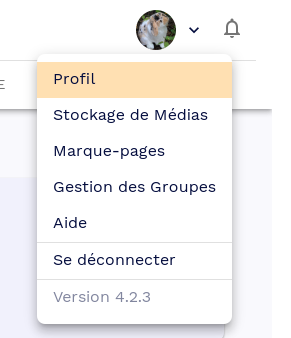
\includegraphics[width=0.3333\linewidth]{./Captures/menu.profil.png}
%	\caption{}
\end{figure}
et cette fois-ci c'est le choix ``Marque-pages'' qui va être choisi. 

\subsection{Descriptif de la fenêtre}
Une fois la ligne cliquée, une zone ressemblant à cet espace, mais vide bien sûr au début, va s'afficher. 
En voici un descriptif rapide.
\begin{figure}
	\centering
	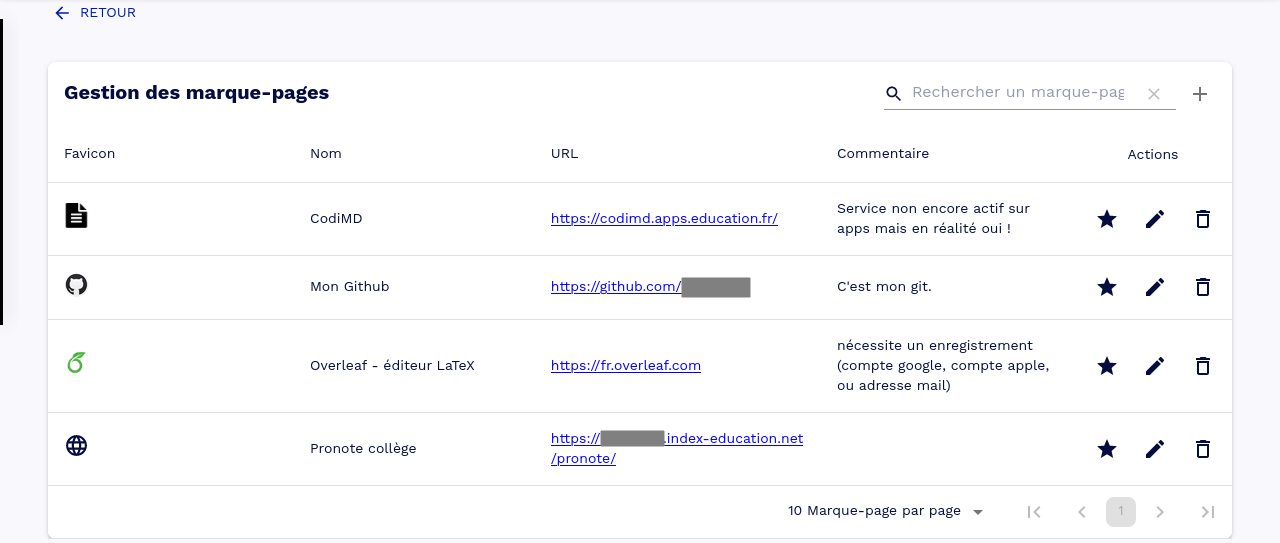
\includegraphics{./Captures/portail.marque.pages.gestion.png}
	\caption{Les marque-pages actuellement saisis dans mon profil}
\end{figure}
\begin{itemize}
	\item Situé en haut à gauche un lien de Retour permet de revenir à l'accueil,
	\item En haut vers la droite, un champ de recherche avec une loupe à sa droite permet de retrouver un lien si vous avez de nombreux liens déjà enregistrés,
	\item tout à droite, un + permet la création d'un nouveau marque page,
	\item la zone centrale affiche, ligne à ligne chaque marque page, les détails sont expliqués là $\rightarrow$ \ref{subsec-detail-bookmark},
	\item en bas à droite une ligne de navigation permet d'aller de page en page ou d'en sélectionner une lorsque beaucoup de liens auront été ajoutés et qu'ils ne tiendront plus sur une ligne unique.
\end{itemize}

\subsection{Détails d'un marque page} \label{subsec-detail-bookmark}
Voici l'examen détaillé d'une ligne de marque-pages, l'exemple du lien vers le site \emph{overleaf}.
\begin{figure}
	\centering
	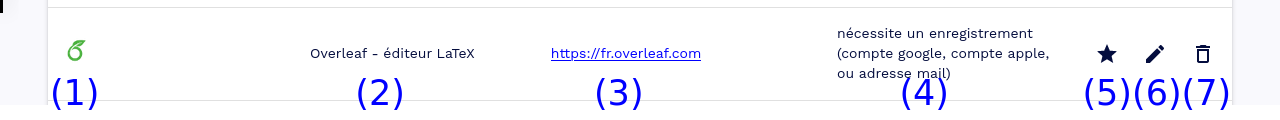
\includegraphics{./Captures/portail.marque.pages.exemple.png}
	\caption{Un exemple de marque-page, vers le site Overleaf}
\end{figure}
La ligne comporte sept zones différentes, voici leur explication de gauche à droite.
\begin{enumerate}
	\item icône du site web en question, sinon un icône générique,
	\item nom donné par moi-même au marque page,
	\item adresse internet du site,
	\item descriptif saisi par moi-même lors de la création du marque page,
	\item marque cet élément comme devant être parmi les favoris donc présent dans la page d'accueil, si l'étoile est creuse, le marque page reste ici, si elle est pleine, alors non seulement il sera présent dans la liste mais aussi apparaîtra en bas de l'onglet d'accueil,
	\item le stylo permet de modifier ultérieurement les détails du marque-page saisis lors de sa création,
	\item comme on peut aisément le deviner, l'icône poubelle permet d'effacer le marque-page, la capture suivante montre d'ailleurs le résultat.
\end{enumerate}
\begin{figure}
	\centering
	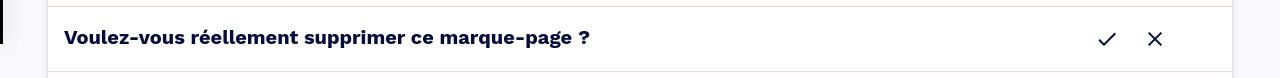
\includegraphics{./Captures/portail.marque.pages.suppression.png}
	\caption{Suppression d'un marque page en attente de ma validation}
\end{figure}
L'appui sur $\surd$ validera l'action de suppression, sur $\times$ vous aurez simplement le retour à la liste des marque pages sans suppression.

De retour à l'écran d'accueil, vous aurez, en bas du profil, tous les marque-pages marqués comme favoris apparaissent.
\begin{figure}
	\centering
	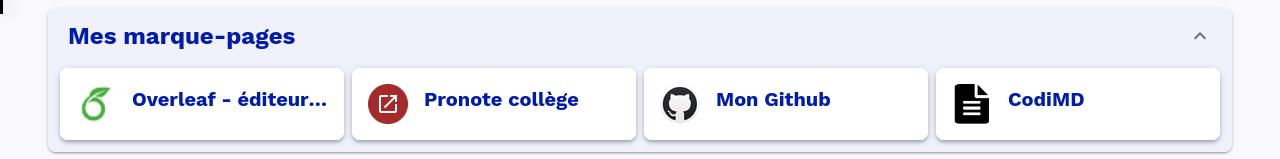
\includegraphics{./Captures/portail.accueil.mes.favoris.png}
	\caption{Mes marque-pages favoris affichés dans le profil.}
\end{figure}

\subsection{Création d'un marque-pages}
En cliquant sur le ``+'' à droite de la zone de recherche, elle-même en haut à droite de la fenêtre, cette mini fenêtre va s'afficher centralement.
\begin{figure}
	\centering
	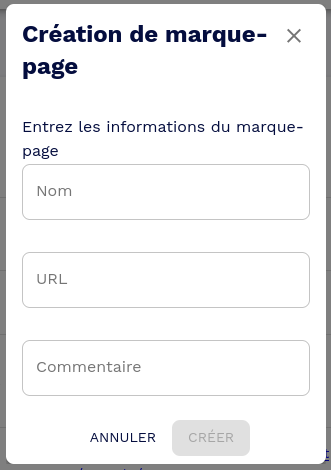
\includegraphics[width=0.333\linewidth]{./Captures/portail.marque.pages.creation.png}
	\caption{Création d'un marque page, pour l'instant vide.}
\end{figure}
Les seules indications importantes consistent à bien remplir tous les champs d'une part et surtout de bien ajouter \texttt{https://} ou \texttt{http://} en début d'adresse, le plus simple étant de copier-coller l'adresse affichée dans la barre éponyme du navigateur internet.